\section{Auswertung}
\label{sec:Auswertung}

% Messwerte: Alle gemessenen physikalischen Größen sind übersichtlich darzustellen.

% Auswertung:
% Berechnung der geforderten Endergebnisse
% mit allen Zwischenrechnungen und Fehlerformeln, sodass die Rechnung nachvollziehbar ist.
% Eine kurze Erläuterung der Rechnungen (z.B. verwendete Programme)
% Graphische Darstellung der Ergebnisse

\subsection{Bestimmung der Zeitkonstante bei angelegter Rechteckspannung}
\label{sec:Auswertung_Rechteckspannung}

Im ersten Teil des Versuchs, wie in \autoref{sec:Durchführung_1} beschrieben, kann nur ein Foto der Entladekurve als Messergebnis dienen, dieses ist in \autoref{fig:foto_entladekurve} dargestellt.

\begin{figure}
    \centering
    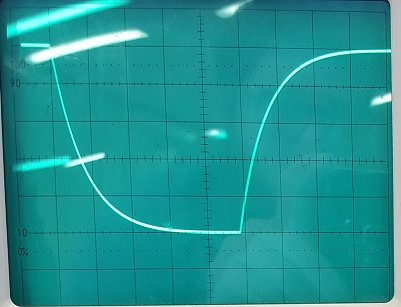
\includegraphics[width=\textwidth/2]{images/foto_01_ausschnitt.jpg}
    \caption{Foto der Entladekurve des RC Glieds bei angeschlossener Rechteckspannung mit $\SI{100}{\hertz}$ wobei die x-Achse auf $\SI{1}{\milli\second}$ und die y-Achse auf $\SI{0.2}{\volt}$ geregelt ist}
    \label{fig:foto_entladekurve}
\end{figure}

\begin{table}
    \centering
    \caption{Abgelesene Werte aus \autoref{fig:foto_entladekurve} mit y-Achse als Kondensatorspannung $U_C$ und x-Achse als Zeit $t$}
    \label{tab:entladekurve}
    \begin{tabular}{c c}
        \toprule
        \tableSI{U_C}{\volt} & \tableSI{t}{\milli\second} \\
        \midrule
        1.00 & 0.00 \\
        0.90 & 0.10 \\
        0.80 & 0.20 \\
        0.70 & 0.30 \\
        0.60 & 0.40 \\
        0.50 & 0.50 \\
        0.44 & 0.60 \\
        0.40 & 0.70 \\
        0.36 & 0.80 \\
        0.28 & 1.00 \\
        0.20 & 1.20 \\
        0.16 & 1.40 \\
        0.12 & 1.60 \\
        0.08 & 1.80 \\
        0.06 & 2.00 \\
        0.04 & 2.30 \\
        0.02 & 2.70 \\
        \bottomrule
    \end{tabular}
\end{table}

Wenn die Werte aus \autoref{tab:entladekurve} nun als Graph mit y-Achse $\ln\left( \frac{U_C}{U_0} \right)$ dargestellt werden, entsteht \autoref{fig:entladekurve_plot}, wobei $U_0=\SI{1}{\volt}$ ist.

\begin{figure}
    \centering
    \includegraphics[width=\textwidth]{build/plot_entladekurve.pdf}
    \caption{Graph der Werte aus \autoref{tab:entladekurve} und der passenden Ausgleichsgerade}
    \label{fig:entladekurve_plot}
\end{figure}

Diese Darstellung entspricht der Gleichung 
\begin{equation}
    \ln\left(\frac{U_C}{U_0}\right) = -\frac{t}{RC}
\end{equation}
wie aus \autoref{eq:entladungsladung} zu sehen ist.
Die entsprechende Ausgleichsgerade wurde in Python mit der Bibliothek SciPy\cite{scipy} mit
\begin{equation}
    f(x)=ax+b
\end{equation}
berechnet.
Wobei sich hier eine Steigung von $a = \SI{-1431+-19}{\second}^{-1}$ ergibt. 
Damit lässt sich die Zeitkonstante als 
\begin{equation}
    RC = \SI{0.6988+-0.0092}{\milli\second}
\end{equation}
bestimmen.

\subsection{Bestimmung der Zeitkonstante bei angelegter Sinusspannung}
\label{sec:Auswertung_Sinusspannung}

Die Ergebnisse der im \autoref{sec:Durchführung_2} beschriebenen Durchführung sind in \autoref{tab:gemessen} dargestellt. Hierbei ist zu beachten, dass die Werte $a_{\text{gemessen}}$ bei einer invertierten Generatorspannung abgelesen wurden. Also entspricht der zeitliche Abstand $a_{\text{gemessen}}$ der Zeit zwischen steigendem Nulldurchgang der Kondensatorspannung und abfallendem Nulldurchgang der Generatorspannung.
Somit ergeben sich die für \autoref{eq:phasenverschiebung2} gesuchten $a$ durch
\begin{equation}
    a = \frac{1}{2f} - a_{\text{gemessen}}.
\end{equation}

\begin{table}
    \centering
    \caption{Messergebnisse zu \autoref{sec:Durchführung_2} mit Generatorfrequenz $f$, Kondensatorspannung $U_C$, zeitlichen Abständen $a_{\text{gemessen}}$ und $a$}
    \label{tab:gemessen}
    \begin{tabular}{c c c c}
        \toprule
        \tableSI{f}{\hertz} & \tableSI{U_C}{\volt} & \tableSI{a_{\text{gemessen}}}{\milli\second} & \tableSI{a}{\milli\second} \\
        \midrule
        20 & 1.000 & 25.000 & 0.000 \\
        50 & 0.960 & 9.200 & 0.800 \\
        100 & 0.900 & 4.200 & 0.800 \\
        200 & 0.700 & 1.850 & 0.650 \\
        300 & 0.550 & 1.150 & 0.517 \\
        400 & 0.450 & 0.800 & 0.450 \\
        500 & 0.360 & 0.620 & 0.380 \\
        600 & 0.300 & 0.500 & 0.333 \\
        800 & 0.240 & 0.360 & 0.265 \\
        1000 & 0.200 & 0.280 & 0.220 \\
        2000 & 0.100 & 0.130 & 0.120 \\
        3000 & 0.067 & 0.085 & 0.082 \\
        4500 & 0.044 & 0.056 & 0.055 \\
        6000 & 0.034 & 0.042 & 0.041 \\
        10000 & 0.020 & 0.025 & 0.025 \\
        \bottomrule
    \end{tabular}
\end{table}

\begin{figure}
    \centering
    \includegraphics[width=\textwidth]{build/plot_spannungen.pdf}
    \caption{Graph des Spannungsverhältnises $U_C/U_0$ in Abhängigkeit zur Generatorfrequenz $f$ aus der \autoref{tab:gemessen} wobei die Generatorspannung konstant auf \SI{1}{\volt} bleibt}
    \label{fig:plot_spannungen}
\end{figure}

Durch die Gleichung
\begin{equation}
    \frac{U_C}{U_0} = \frac{1}{\sqrt{1+(2 \pi f)^2R^2C^2}}
\end{equation}
lässt sich nun die Zeitkonstante $RC$ bestimmen indem eine Ausgleichsrechnung wie in \autoref{fig:plot_spannungen} mit
\begin{equation}
    f(x) = \frac{1}{\sqrt{1+(2 \pi x)^2a^2}}
\end{equation} 
ausgeführt wird. Diese Ausgleichsrechnung wurde mit der Python Bibliothek SciPy\cite{scipy} ausgeführt und ergibt die Zeitkonstante
\begin{equation}
    RC = \SI{0.8078+-0.0056}{\milli\second}.
\end{equation}

Eine weitere Möglichkeit die Zeitkonstante zu berechnen ist mithilfe der frequenzabhängigen Phase $\varphi$ zwischen Generator- und Kondensatorspannung. Diese lässt sich über \autoref{eq:phasenverschiebung2} berechnen. Die so berechneten $\varphi$ sind in \autoref{tab:phasen} gelistet.

\begin{table}
    \centering
    \caption{Generatorfrequenz $f$, Kondensatorspannung $U_C$ und die mit $a$ berechnete Phasenverschiebung $\varphi$}
    \label{tab:phasen}
    \begin{tabular}{c c c}
        \toprule
        \tableSI{f}{\hertz} & \tableSI{U_C}{\volt} & \tableSI{\varphi}{\radian} \\
        \midrule
        20 & 1.000 & 0.000 \\
        50 & 0.960 & 0.251 \\
        100 & 0.900 & 0.503 \\
        200 & 0.700 & 0.817 \\
        300 & 0.550 & 0.975 \\
        400 & 0.450 & 1.131 \\
        500 & 0.360 & 1.194 \\
        600 & 0.300 & 1.255 \\
        800 & 0.240 & 1.332 \\
        1000 & 0.200 & 1.382 \\
        2000 & 0.100 & 1.508 \\
        3000 & 0.067 & 1.546 \\
        4500 & 0.044 & 1.555 \\
        6000 & 0.034 & 1.546 \\
        10000 & 0.020 & 1.571 \\
        \bottomrule
    \end{tabular}
\end{table}

\begin{figure}
    \centering
    \includegraphics[width=\textwidth]{build/plot_phasen.pdf}
    \caption{Die Phasenverschiebung $\varphi$ zur Generatorfrequenz $f$ aus \autoref{tab:phasen} abgebildet}
    \label{fig:plot_phasen}
\end{figure}

Die mithilfe von SciPy\cite{scipy} und
\begin{equation}
    f(x)=-arctan(-2\pi f a)
\end{equation}
erstellte Ausgleichsrechnung ergibt nach \autoref{eq:phasenverschiebung} eine Zeitkonstante
\begin{equation}
    RC = \SI{0.8258+-0.0261}{\milli\second}.
\end{equation}

Die Kondensatorspannung $U_C$ wird nun in einem Polarkoordinatensystem in Abhängigkeit der Phase $\varphi$ dargestellt. Die gemessenen Werte sind aus \autoref{tab:phasen} abzulesen und die erwartete Kurve wird nach \autoref{eq:spannung_phase} berechnet.

\begin{figure}
    \centering
    \includegraphics[width=\textwidth]{build/plot_polar.pdf}
    \caption{Kondensatorspannung $U_C$ in Abhängigkeit von der Phase $\varphi$ entnommen aus \autoref{tab:phasen}}
    \label{fig:plot_polar}
\end{figure}

\subsection{Betrachtung des RC-Glieds als Integrator}
\label{sec:Auswertung_Integrator}

Im letzten Teil des Versuchs wie in \autoref{sec:Durchführung_3} beschrieben sind die Ergebnisse nur in Form von Fotos darzustellen. Diese sind in \autoref{fig:fotos_integrator} zu sehen. Hierbei wurde jeweils die Generatorfrequenz von $\SI{5}{\kilo\hertz}$ gewählt und sowohl die Generatorspannung als auch die Kondensatorspannung abgebildet.

\begin{figure}
    \centering
    \begin{subfigure}{0.3\textwidth}
        \centering
        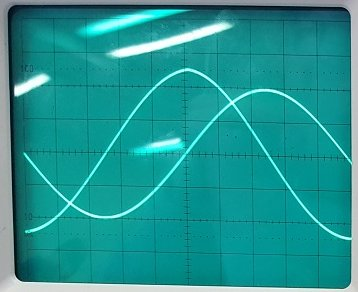
\includegraphics[height=3.3cm]{images/foto_03_ausschnitt.jpg}
        \caption{Sinusspannung}
        \label{fig:foto_sin_integrator}
    \end{subfigure}
    \begin{subfigure}{0.3\textwidth}
        \centering
        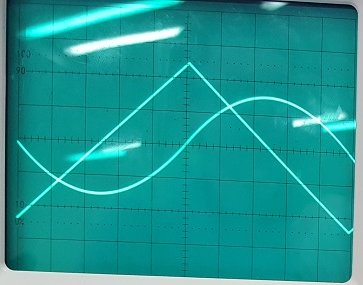
\includegraphics[height=3.3cm]{images/foto_04_ausschnitt.jpg}
        \caption{Sägezahnspannung}
        \label{fig:foto_saege_integrator}
    \end{subfigure}
    \begin{subfigure}{0.3\textwidth}
        \centering
        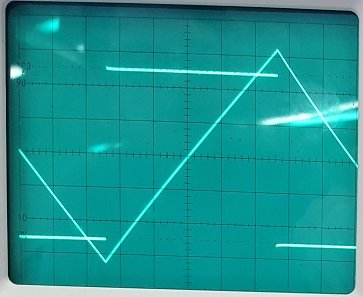
\includegraphics[height=3.3cm]{images/foto_05_ausschnitt.jpg}
        \caption{Rechteckspannung}
        \label{fig:foto_rechteck_integrator}
    \end{subfigure}
    \caption{Fotos der Integratorschaltung für eine Generatorfrequenz von $\SI{5}{\kilo\hertz}$ und verschiedene Generatorspannungstypen}
    \label{fig:fotos_integrator}
\end{figure}

Hier ist zu sehen, dass die angelegte Spannung integriert wird. Eine Sinusspannung wird zu einer Sinusspannung um $\pi/2$ verschoben, eine Sägezahnspannung wird zu einer parabolischen Spannung und eine Rechteckspannung wird zu einer Sägezahnspannung.